\documentclass[aspectratio=169]{beamer}
\usetheme{Madrid}
\usepackage[utf8]{inputenc}
\usepackage[T1]{fontenc}
\usepackage{tikz}
\usepackage{amssymb}
\usepackage{graphicx}
\setbeamertemplate{navigation symbols}{}
\setbeamercolor{title}{fg=white,bg=violet!70!purple}
\setbeamercolor{frametitle}{fg=white,bg=violet!70!purple}
\setbeamercolor{block title}{bg=violet!70!purple!20,fg=black}
\setbeamercolor{block body}{bg=violet!70!purple!8,fg=black}
\setbeamercolor{item}{fg=violet!70!purple}
\setbeamercolor{itemize item}{fg=violet!70!purple}
\setbeamertemplate{itemize item}[triangle]

\title{Story Studio 3 — Make It Click}
\subtitle{onclick — a button that actually does something when pressed}
\author{ByteForge --- Grade 7 --- Game Maker}
\date{}

\begin{document}

\begin{frame}
    \titlepage
\end{frame}

\begin{frame}{Today's Plan}
    \begin{itemize}
        \item Click to Reveal
        \item Click for More
        \item Both at Once
        \item Button Talks Back
        \item[$\bigstar$] BOSS --- The Big Reveal
    \end{itemize}
\end{frame}

\begin{frame}{onclick — code that waits for a click}
    \large
    \begin{itemize}
        \item Every block before this ran the instant you pressed Run. "When button is clicked" waits, doing nothing, until a real click happens.
        \item Worked example: nothing inside "when button is clicked" runs when you press Run — it only runs the moment a real click happens, which is why the checker fires one simulated click to test it.
    \end{itemize}

    \begin{center}
    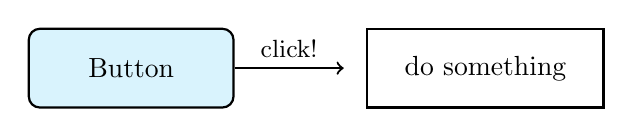
\begin{tikzpicture}[scale=0.9]

        \node[draw, thick, rounded corners, minimum width=2.6cm, minimum height=1cm, fill=cyan!15] (btn) at (0,0) {Button};
        \draw[->, thick] (btn) -- (3,0) node[midway, above] {\small click!};
        \node[draw, thick, minimum width=3cm, minimum height=1cm] (act) at (5,0) {do something};
    \end{tikzpicture}
    \end{center}
\end{frame}


\begin{frame}{The same event, a different action}
    \large
    \begin{itemize}
        \item The event ("when clicked") stays the same
        \item What happens inside it is entirely up to you.
    \end{itemize}
\end{frame}


\begin{frame}{One event, multiple actions}
    \large
    \begin{itemize}
        \item Anything placed inside "when clicked" all runs together, in order, from a single click
        \item No limit to how many blocks you can stack.
    \end{itemize}
\end{frame}


\begin{frame}{A button can change itself}
    \large
    \begin{itemize}
        \item It's easy to assume a button can only affect OTHER things
        \item But it can just as easily change its own label.
    \end{itemize}
\end{frame}


\begin{frame}{BOSS — structure, style, and behaviour}
    \large
    \begin{itemize}
        \item Week 1 gave structure, Week 2 gave style, Week 3 gives BEHAVIOUR
        \item The same three-part split every real website is built from.
    \end{itemize}
\end{frame}

\begin{frame}{Real-World Examples}
    \large
    \begin{itemize}
        \item Click an "Add to cart" button on a real shopping site
        \item The label changing to "Added \textbackslash\{\}checkmark" or a counter updating is exactly this week's "button talks back" idea, live in production software. A Minecraft crafting-table "craft" button is the same: click it, and it visibly does something (moves items) right there.
    \end{itemize}
\end{frame}


\begin{frame}{Image}
    \begin{center}
    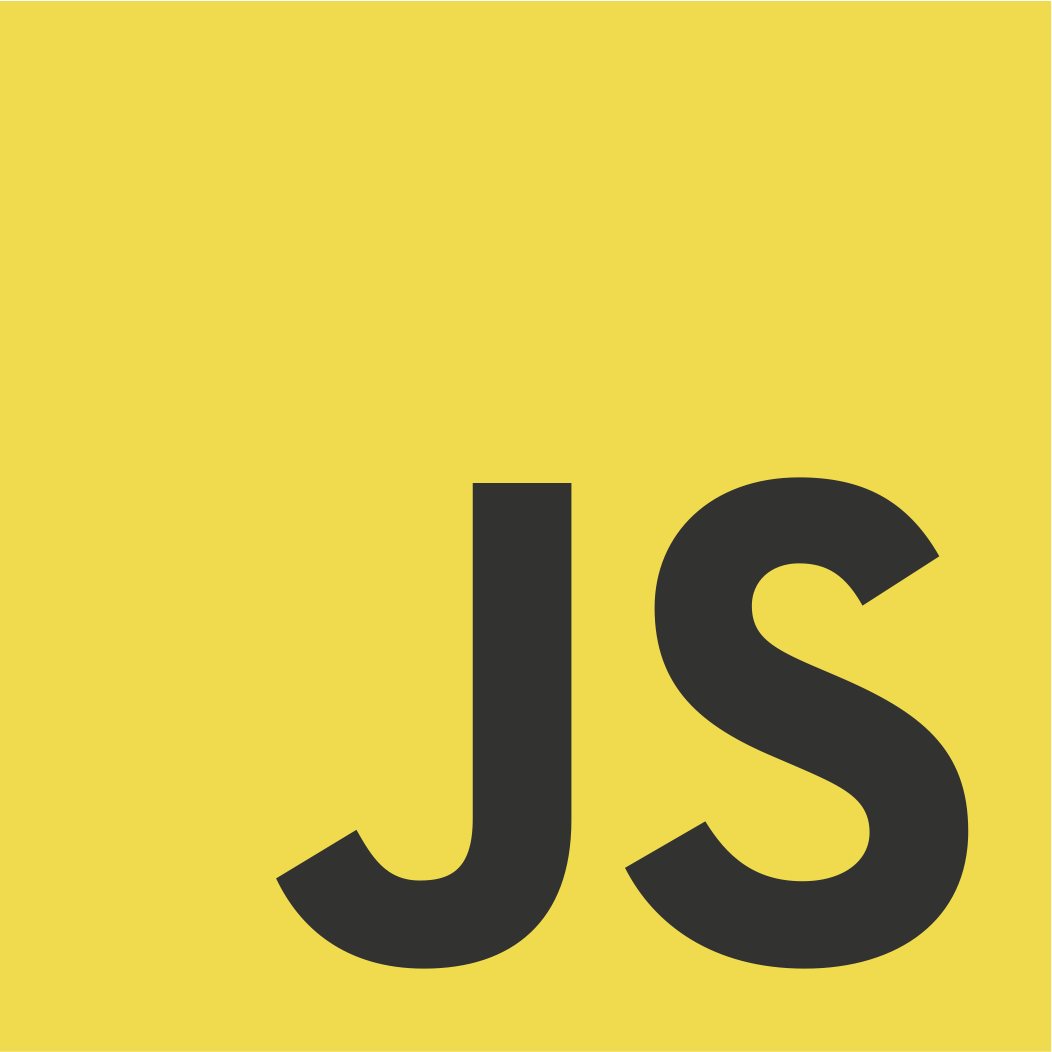
\includegraphics[width=0.5\textwidth]{images/js.png}

    \large The real language behind onclick --- what you just built with blocks.

    \small JavaScript logo — Chris Williams, public domain, via Wikimedia Commons
    \end{center}
\end{frame}

\begin{frame}{Let Them Discover}
    \Large
    Find a button on any app or website that changes itself when clicked (a like button, a "show password" eye icon, a checkbox). What exactly changes — text, colour, icon? Nothing else on the page needs to change too.
\end{frame}

\begin{frame}{Your Turn}
    \Large
    Open the student map, find \textbf{Story Studio 3 — Make It Click}, and work through it
    hands-on --- everything you just saw, they now do themselves.
\end{frame}

\end{document}
